

\chapter{\texorpdfstring{The hardness of the \ce{Ti2Ni} structure}{The hardness of the Ti2Ni structure}}
\graphicspath{{hardness_of_ti_2_ni/Figs/}}
\label{chap:ti2ni_hardness}



The previous chapters have explained observations of dislocations in almost ideal model systems, the alkali halides and the MAX phases, but the question remains as to whether these models of dislocation motion are applicable more broadly, and specifically to systems with a greater industrial relevance. A candidate system must fit some criteria: The MAX phases can accommodate chemically, and hence elastically, heterogeneous regions because the unit cells are large, at least parallel the $c$ axis, so the unit cell of any candidate must be large, of the order of \SI{10}{\angstrom}. The MAX phases show very easy basal slip but slip out of the basal plane is much harder, so any candidate phase will have higher crystal symmetry and must have enough independent slip systems to allow full plasticity. The MAX phases also allow a large range of heterogeneity to be investigated due to the wide range of stable compositions, so a range of alloying possibilities is necessary to investigate this softening effect based on elastic heterogeneity.

The \ce{Ti2Ni} structure was selected because it meets all of these criteria to an adequate extent. The structure is an FCC crystal structure (Fd\={3}m) with 96 atoms in the unit cell and, for the case of titanium and nickel, a lattice parameter of \SI{11.28}{\angstrom} \cite{Yurko1959,Yurko1962}. The range of elements that can be incorporated into the structure is also large, a search using the Inorganic Crystal Structure database \cite{ICSD} returned 103 results including elements such as sodium, zinc, germanium, niobium and hafnium, amongst others.

\section{The \texorpdfstring{\ce{Ti2Ni}}{Ti2Ni} structure}
\FloatBarrier


Phases with the \ce{Ti2Ni} structure is a large unit cell with a large number of atoms and appears complex, a plan view is shown in \autoref{fig:Ti2Ni_plan}. However the symmetry of the structure is high, the space group is Fd\={3}m, and there are only three distinct sites; the wyckoff positions for which are 16(c) (Ti1), 32(e) (Ni) and 48(f) (Ti2), which have the coordination numbers 12, 12 and 14 respectively. The packing and ordering of these clusters creates the face-centred symmetry. The creation of a face-centred structure, rather than an icosahedral packing, requires distorted icosahedral coordination polyhedra.


\begin{figure}[h]
\centering
\includegraphics[width=0.5\textwidth]{Ti2Ni_structure}
\caption[Plan view of the \ce{Ti2Ni} structure.]{Plan view of the \ce{Ti2Ni} structure down the [001]. The blue atoms are titanium sites and the silver atoms are nickel sites.\label{fig:Ti2Ni_plan}}
\end{figure}



While in many phases descriptions of structures the clusters are little more than geometrically elucidating \cite{Steurer2006}, in the \ce{Ti2Ni} phases there is direct evidence that the bonding and properties are highly localised into the clusters, particularly the 16(c) site, at which a titanium atom sits \cite{Ivanovic2006}. \citet{Ivanovic2006} report the electric field gradient of the material to be extremely heterogeneous, showing different bonding at the two titanium sites, the 16(c) and the 48(f), just \SI{3}{\angstrom} apart. 

The 16(c) coordination cluster is found to be the most stable and to have a metallic character to its bonding. The cluster at the 32(e) site is less stable but has otherwise similar character to the coordination cluster at 16(c), its appearance in both the \ce{Ti2Ni} structure and in a related quasicrystal imply this is a natural geometric complement to the 16(c) cluster, i.e. the two arrangements pack well. The 48(f) arises in the crystalline state but not the quasicrystalline state, and so must be a product of space filling in the \ce{Ti2Ni} crystal structure. The 48(f) cluster shows a large variation bond lengths among bonds of the same type; \citet{Ivanovic2006} ascribe this to more covalent and weaker bonding.


The details of the bonding are not of primary interest however, rather how these relate to dislocation motion. Here we must consider broader regions of crystal rather than local clusters. If the clusters are physically significant structural units then the way these pack together will be key to the dislocation properties, just as in close-packed metals the way atoms pack together is key to the character the dislocations. The 16(c) sites form chains, sharing faces and defining a tetrahedron within the unit cell. This is in fact a Kagom\'{e} net, exactly as exists in the Laves phases \cite{Stein2004,Stein2005}, which are planes parallel to the \{111\} planes. The distinction is that the Kagom\'{e} net in the Laves phases are defined by single atomic sites rather than clusters. The Kagom\'{e} network of 16(c) clusters is shown in \autoref{fig:16c_network_Ti2Ni}

\begin{figure}
\centering
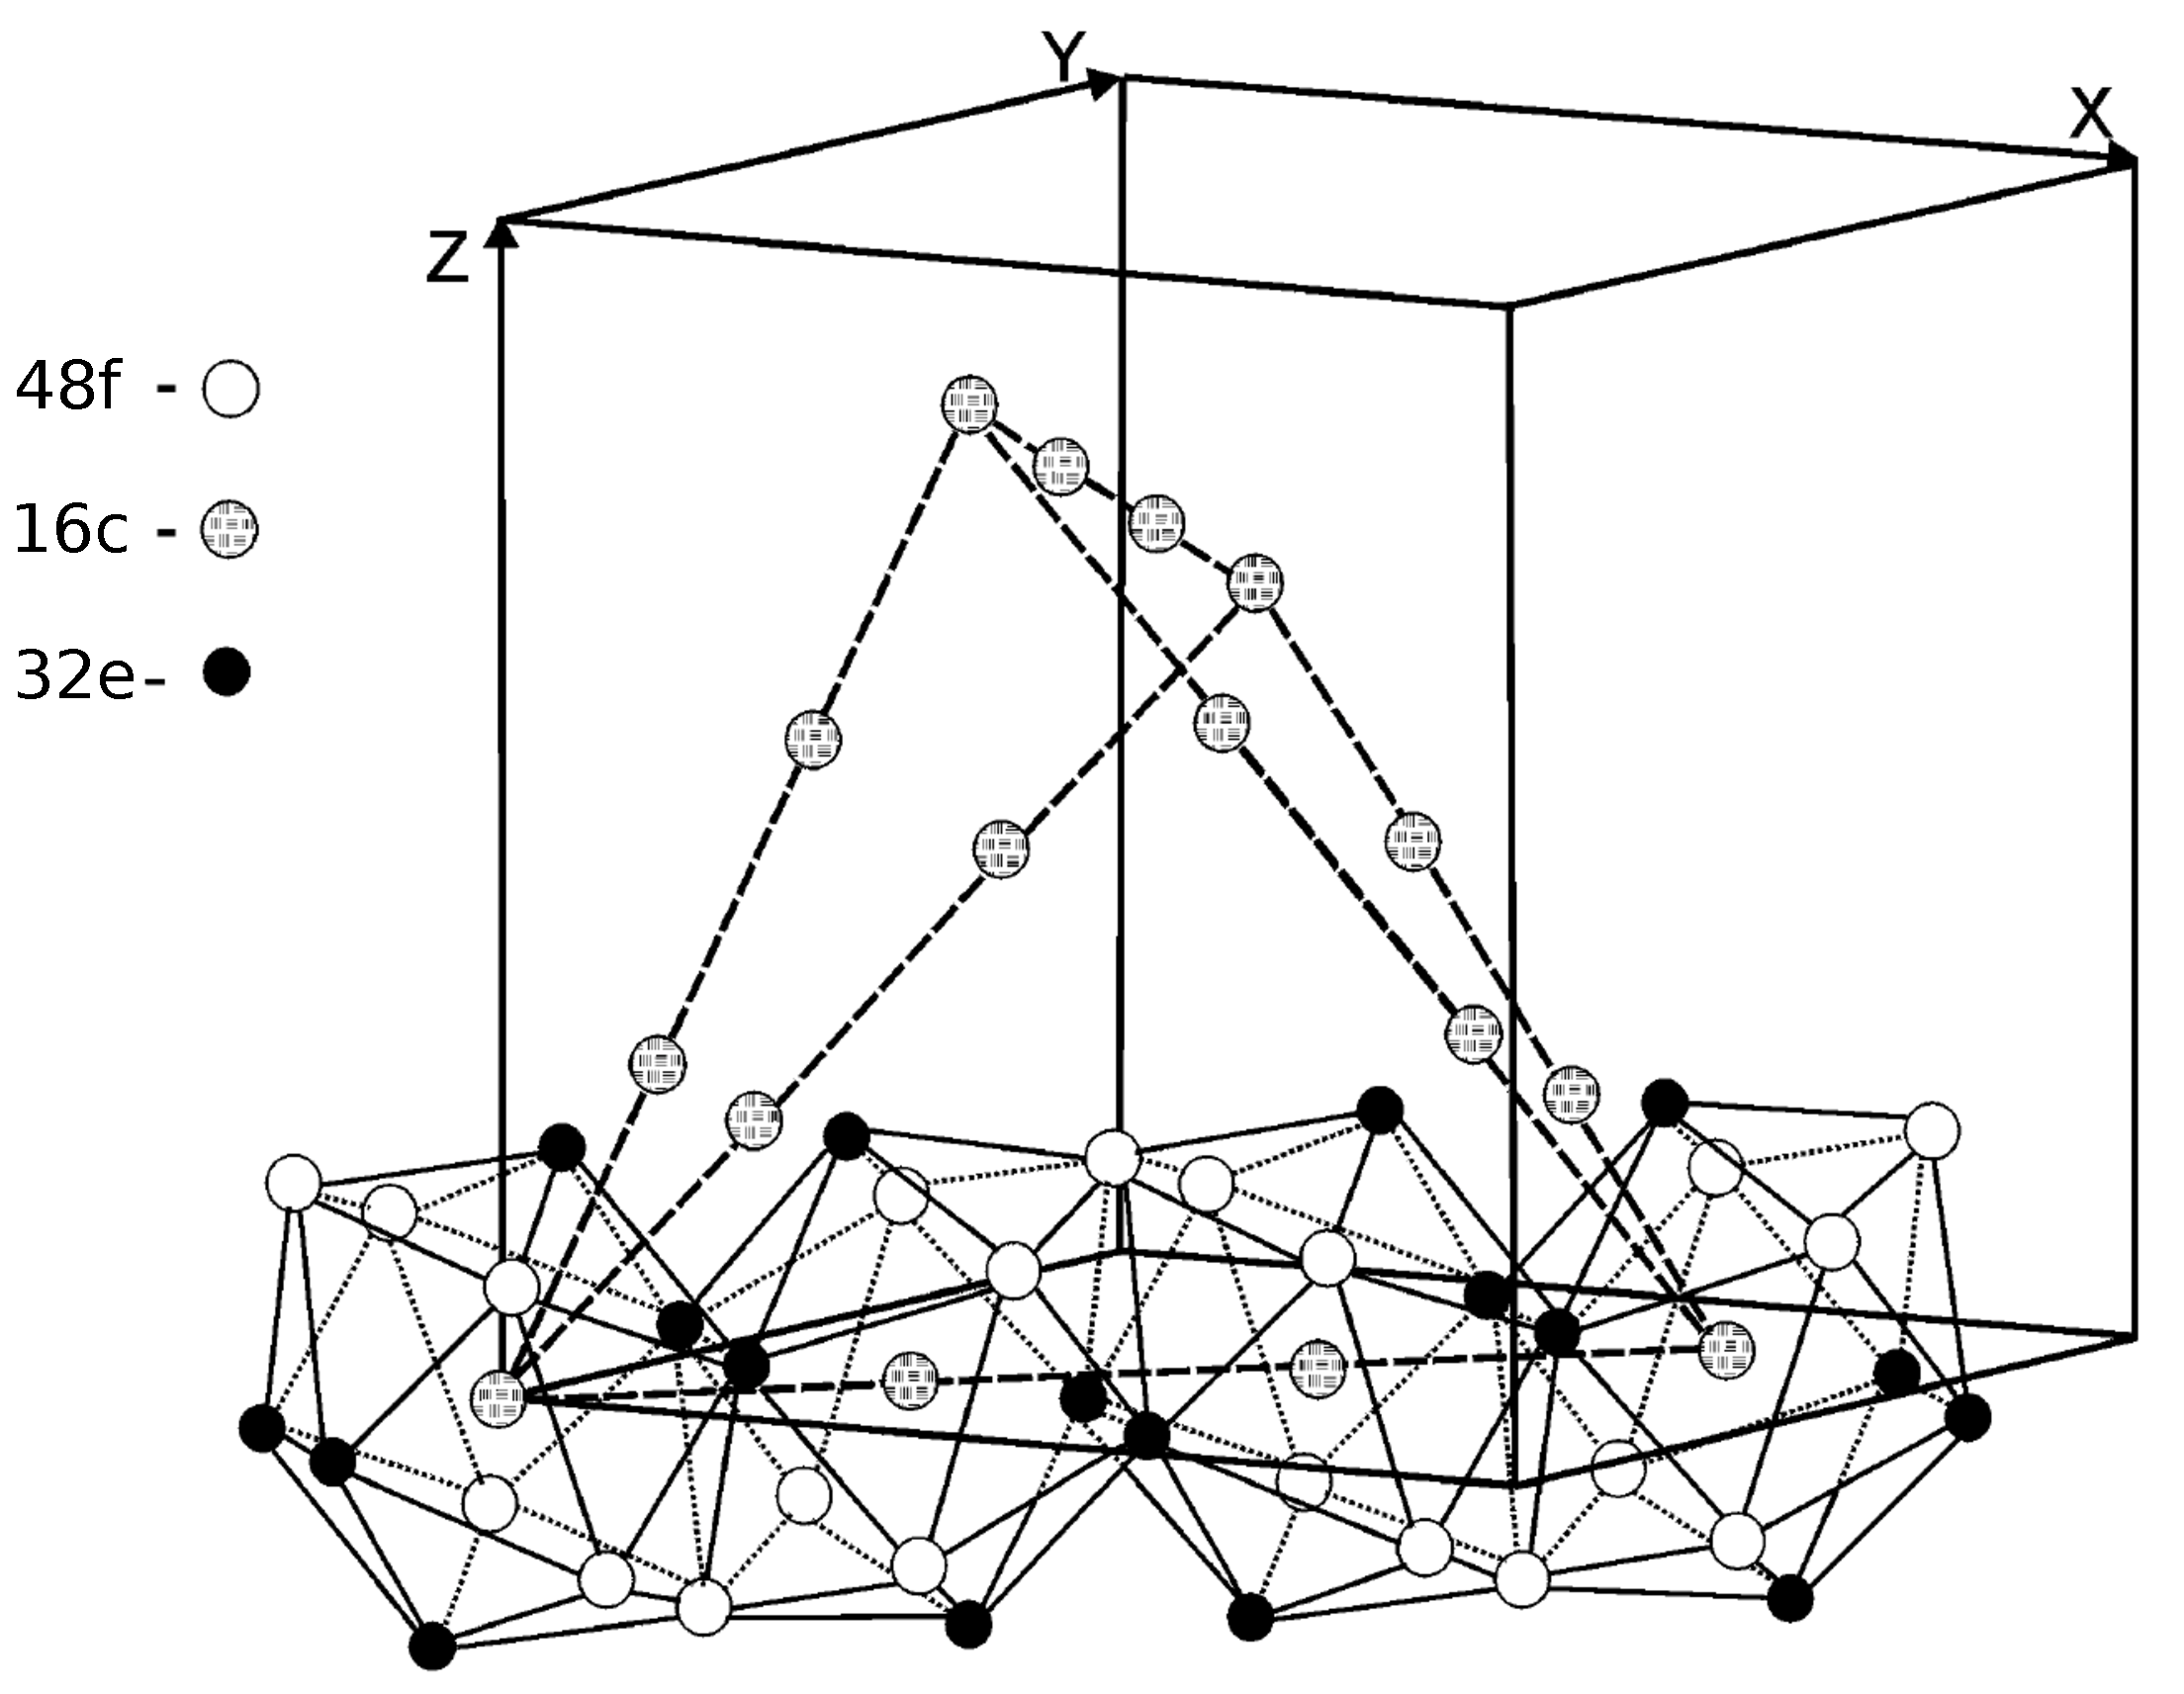
\includegraphics[width=0.5\textwidth]{Ti2Ni_16c_sites}
\caption[The Kagom\'{e} network formed by atomic clusters around the 16(c) site.]{The network formed by the metallically bonded coordination clusters at the 16(c) site in the \ce{Ti2Ni} structure, reproduced from \cite{Ivanovic2006}.\label{fig:16c_network_Ti2Ni}}
\end{figure}


Dislocations are long, linear defects and so will respond to the properties of extended regions of a crystal. In other face-centred cubic intermetallics with large unit cells slip has been shown to be on the \{111\} planes and in either <1\={1}0> or <11\={2}> directions, in a simple analogy with FCC metals \cite{Davis2015}. The \{111\} planes are shown in \autoref{fig:Ti2Ni_111_planes}. It is clear that the heterogeneity inherent in the crystal is relevant to the slip system that is likely to operate in this structure since there are distinct layers in the structure when viewed in this way. The view in \autoref{fig:Laves_phase_Ti2Ni_similarity} shows a marked similarity with the Laves phase structure which similarly has a Kagom\'{e} layer and a puckered triple layer, albeit with shorter repeat distances. An important point is that the Kagom\'{e} layer formed by the 16(c) clusters is potentially physically significant within the crystal structure; the crystal can then be considered a network of intersecting Kagom\'e layers containing all of the 16(c) (Ti1) sites, all of the 32(e) (Ni) sites and a number of the 48(f) (Ti2) sites in the crystal and the space between is filled by the remaining 48(f) (Ti2) sites.


\begin{figure}
\centering
\begin{subfigure}{0.65\textwidth}
\centering
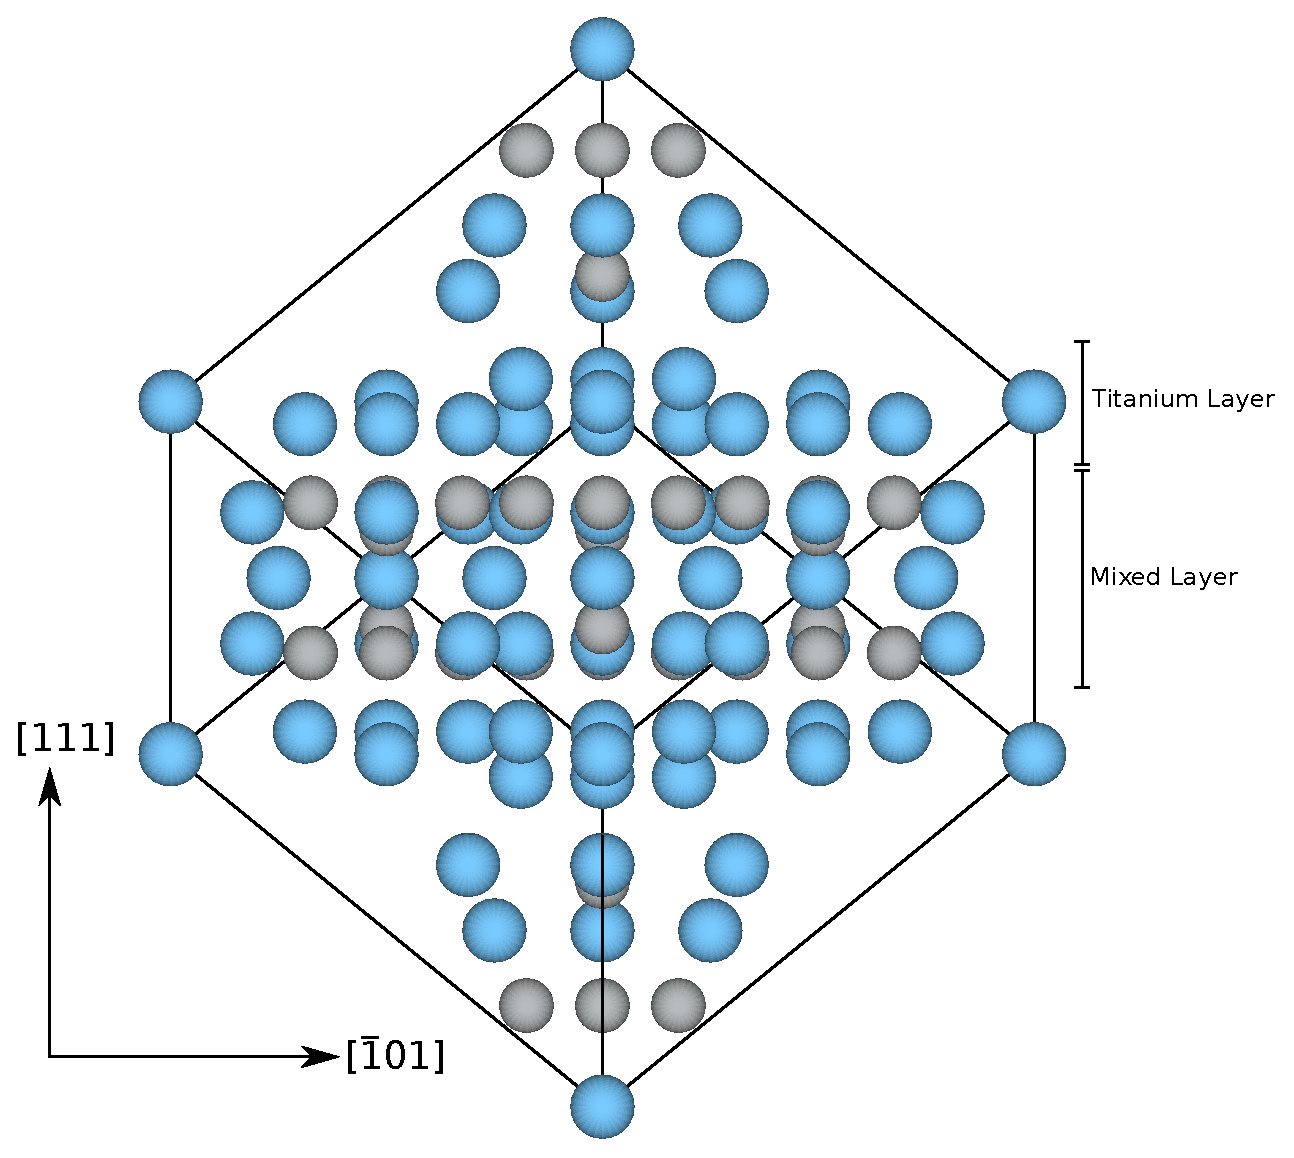
\includegraphics[width=\textwidth]{Ti2Ni-slip_system}
\caption{A view of the \ce{Ti2Ni} unit cell showing the \{111\} planes with the ``ideal'' burgers vector across the diagram.\label{fig:slip_system_Ti2Ni}}
\end{subfigure}

\begin{subfigure}{0.65\textwidth}
\centering
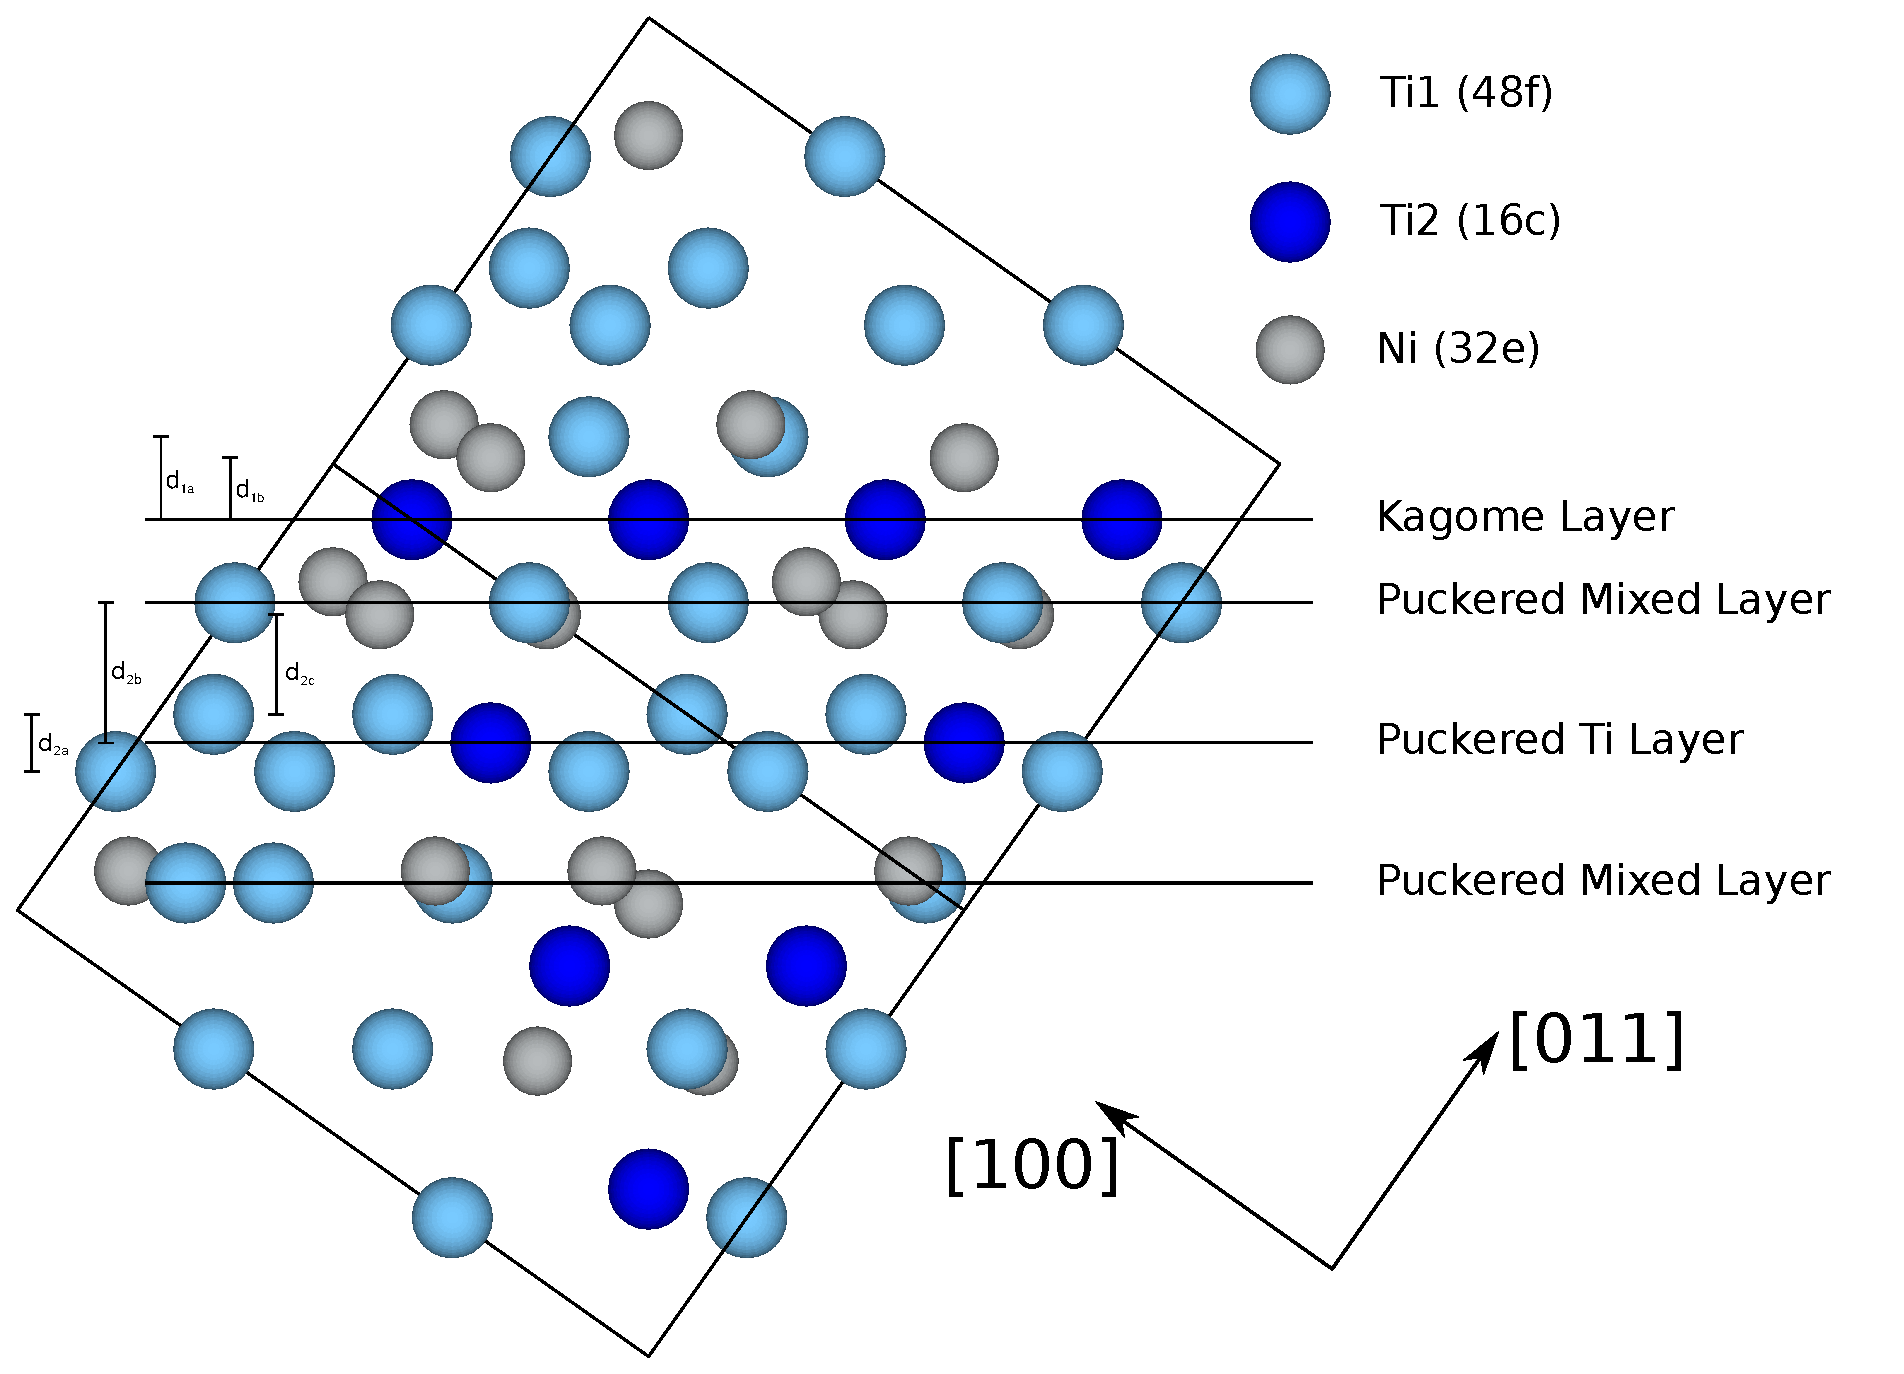
\includegraphics[width=\textwidth]{Ti2Ni-layers}
\caption{A view of the \ce{Ti2Ni} structure showing the \{111\} planes looking down the <\=101> direction.\label{fig:Laves_phase_Ti2Ni_similarity}}
\end{subfigure}
\caption[The \{1\,1\,1\} planes of the \ce{Ti2Ni} structure.]{The \{111\} layers of the \ce{Ti2Ni} structure projected along two different directions.\label{fig:Ti2Ni_111_planes}}
\end{figure}

\subsection{The alloying additions and effects}

To assess the effect of alloying additions on the dislocations salient regions of the crystal structure must be considered, at least to a degree; plainly the situation for \ce{Ti2Ni} is not as simple and clear cut as the MAX phases considered in \autoref{chap:dislocations_in_max_phases}, which have a very simple layered structure. Much of this complexity arises because any plane in a face-centred cubic structure will necessarily have a high multiplicity and so intersect with other planes of the same kind.

A simple model of the regions relevant to dislocations is shown in \autoref{fig:slip_system_Ti2Ni}, where distinct layers are labelled showing a mixture of titanium and nickel in one region (the 16(c) clusters) and a purely titanium region in the other. These two layers together form one complete \{111\} layer which is then stacked in the familiar ...ABCABC... sequence to form the structure, so this description includes all the atoms of the structure.

The atom on the nickel site is usually the more electronegative, at least in the alloys considered here, and these sites are associated with the 16(c) cluster which is more strongly bonded than the other clusters as would be expected. The ratio of Ni:Ti in the mixed region is 9:8, so the parallel to the electronegativity difference for the MAX phases, \autoref{eqn:MAX_electronegativity_diff}, is
\begin{align}
\Delta \chi &= \chi_{\text{mixed}} - \chi_{\text{Ti}} \nonumber\\
\Delta \chi &= \frac{9\chi_{\text{Ni}} + 8\chi_{\text{Ti}}}{17} - \chi_{\text{Ti}}
\end{align}
so variations in the elemental electronegativity will have a smaller effect on the electronegativity difference between the layers due to this mixture of elements in one of the layers.

The \ce{Ti2Ni} structure can accommodate a wide variety of elements but for ease of processing and material availability the compositions were limited to those given in \autoref{tab:compositions_Ti2Ni}. The relevant phase diagrams are given in \autoref{chap:phase_diagrams}.

\FloatBarrier
\begin{table}[!ht]
\centering
\begin{tabular}{|l | c|}
\hline
Stoichiometry & $\Delta \chi$ (\si{\electronvolt}) \\
\hline
\ce{Ti2Ni} \rule{0pt}{3ex}  & 0.444 \\
\ce{Ti2Co} & 0.383 \\
\ce{Hf2Co} & 0.378 \\
\ce{Ti2(Co,Ni)} & 0.414 \\
\ce{(Hf,Ti)_{2}Ni} \rule[-1ex]{0pt}{0pt} & 0.4403 \\
\hline
\end{tabular}
\captionsetup{width=0.5\textwidth}
\caption[Compositions of the investigated \ce{Ti2Ni} phases.]{The compositions used to investigate plasticity in the \ce{Ti2Ni} structure and the corresponding electronegativity (Mulliken scale \cite{Mulliken1934}) difference between the regions shown in \autoref{fig:Ti2Ni_111_planes}. \label{tab:compositions_Ti2Ni}}
\end{table}


\section{Sample preparation}


Samples were prepared by arc melting pieces of the pure elements to form small, roughly cylindrical ingots of around \SI{40}{\gram}. These ingots were then directionally solidified using the optical floating zone technique. 

In the floating zone technique light is focused onto a small region of a prismatic sample to form a molten zone, the  zone is then translated along the length of the sample either by moving the light or by moving the sample. The zone can be passed along the sample once or multiple times in either the same direction or alternating the direction of travel to achieve different ends \cite{Pfann1966}. 

The floating zone furnace used was a FZ-T-12000-X-VPO (Crystal Systems Corp). This system uses four xenon arc lamps, each with an ellipsoidal mirror to focus the light onto the sample, a schematic is shown in \autoref{fig:OFZF_schematic}. The samples were all grown with the seed and feedstock counter rotating at \num{15}~rpm, i.e. \num{30}~rpm relative rotation, and a growth rate of \SI{20}{\milli\meter\per\hour}.


The sample surfaces were ground flat with silicon carbide paper before polishing with a series diamond pastes to a \SI{0.25}{\micro\meter} finish and finally finished with ten minutes of polishing with colloidal silica.


\begin{figure}
\centering
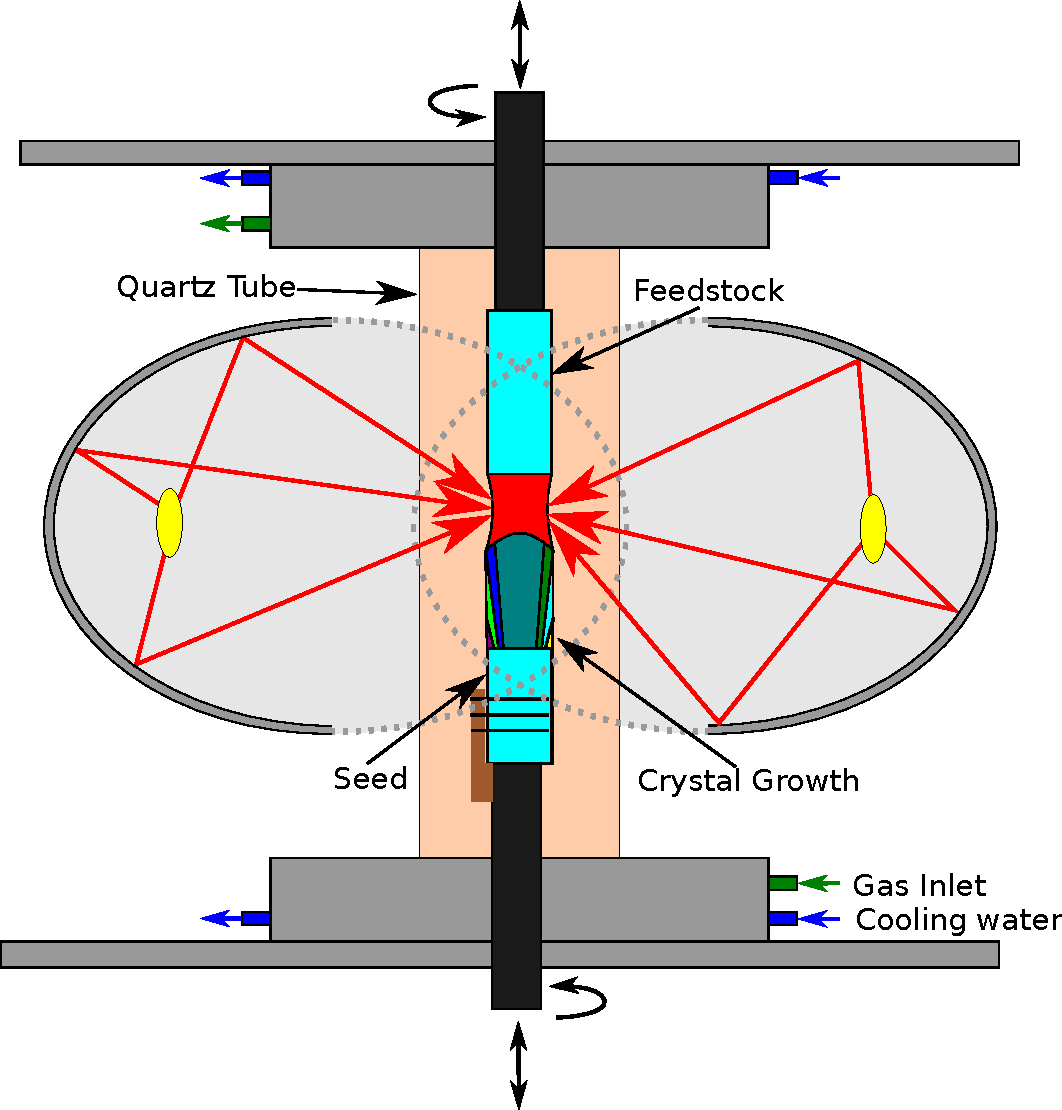
\includegraphics[width=0.6\textwidth]{Image_Furnace_Schematic}
\caption{Schematic of an optical floating zone furnace.\label{fig:OFZF_schematic}}
\end{figure}











%%%%%%%%%%%%%%%%%%%%%%%%%%%%%%%%%%%%%%%%%%%%%%%%%%%%%%%%%%%%%%%%%%%%%%%%%%%%%%%%%%%%%%%%%%%%%%



\section{Mechanical testing}
\label{sec:Ti2Ni_mechtesting}

Investigating the plastic flow of hard materials is a challenging problem which has seen much investigation in recent years. Various techniques exist to investigate plasticity in materials that are likely to fracture in conventional testing, a constraining hydrostatic pressure \cite{Griggs1936,Weinrich1975,Borvin1990}, micropillar compression where the size effects suppress fracture \cite{Uchic2004} or indentation \cite{Cripps2011,tabor2000hardness,Marsh1964,Korte2009}. Of these the indentation hardness test is the simplest. In contrast constraining pressure equipment is complex, the high pressures can induce phase changes and uniaxial properties can only be extrapolated. Micropillar compression, while uniaxial and room temperature, is known to be strongly influenced by size effects \cite{Uchic2004,Greer2005,Greer2006corrigendum}.


When indenting brittle materials small indents are likely to be necessary to suppress cracking, this must be achieved by instrumented indentation, in which the load and the depth are measured during indentation, rather than measuring the area of the residual indent after indentation, however this risks encountering the widely reported indentation size effect \cite{Korte2009,Cripps2011}. To address this the indents must all be the same size, and the samples prepared to the same finish by the same method. The size effect can also be characterised by a set of indents at a range of depths, though identifying the actual causes of the effect is difficult \cite{Korte2009,Cripps2011}.


To ensure that the results from the indent were comparable across the different samples the crystallographic orientation of the grains in the material was identified by electron backscatter diffraction (EBSD) using a Camscan MX2600 FEGSEM and only those grains close to a single zone axis were considered. This ensures that, although the stress state under a Berkovich indenter is complex, the orientation between the stress state and the slip systems is the same for all the indents, thus addressing any Schmid factor effects that might affect the hardness when indenting different crystal faces \cite{Kelly2012ch7}. The <1\,1\,1> was a common growth direction and so only indents into grains oriented within \SI{10}{\degree} of the <1\,1\,1> were used in the analysis, others were discarded.


Indentation was undertaken with the Micromaterials NanoTest indenter using a Berkovich tip. Thermal drift was minimised by heating a chamber containing both the sample and the indenter to \SI{25}{\celsius} and allowing the temperatures to equilibrate over a period of a few hours. The indents were performed under depth control at a loading rate of \SI{5}{\nano\meter\per\second}. To probe the depth dependence of the hardness indents were performed at intervals of c.~\SI{100}{\nano\meter} between \SI{100}{\nano\meter} and \SI{1700}{\nano\meter}. Larger datasets were collected to more accurately determine the hardness on known crystallographic faces, as determined by EBSD. The simplest method to achieve this was to produce a square array of widely spaced indents across the surface and investigate the crystal orientation ex-situ. These indents were performed under the same conditions to a depth of \SI{1}{\micro\meter}.

%%%%%%%%%%%%%%%%%%%%%%%%%%%%%%%%%%%%%%%%%%%%%%%%%%%%%%%%%%%%%%%%%%%%%%%%%%%%%%%%%%%%%%%%%%%

While micropillar compression has not been employed to compare the flow properties of the different phases, the technique has been used to identify the active slip systems of the \ce{Ti2Ni} structure. This can be achieved by milling pillars in an area of the crystal that has been mapped with EBSD. 

Pillars were milled into the sample surface using a focused ion beam microscope (FIB), the system used was a FEI Helios NanoLab with \ce{Ga+} ions operated with the help of Claire Davis \cite{Davis2015} and Robert Jones \cite{Jones2016}. The pillars were milled to be approximately \SI{2}{\micro\meter} in diameter and \SI{5}{\micro\meter} tall. Compression of the micropillars was performed with an in situ Alemnis indenter with a diamond flat punch tip operated by Robert Jones. A detailed description of the experimental and analysis procedures can be found in \cite{Davis2015}.

The slip trace on the pillar can be used to determine the slip plane by comparison with the crystal structure using a visualisation package such as VESTA \cite{Momma2011,Davis2015}. The slip direction can be determined by finding the lattice vector parallel to the lateral (i.e. perpendicular to the compression axis) movement during slip and projecting this onto the slip plane, however this can be difficult in FCC systems where likely slip vectors are relatively close together, e.g. <101> and the <112> \cite{Davis2015}.


\section{Results and Discussion}


\subsection{Size effect}


The size effect was investigated first, the results for \ce{Ti2Ni} and \ce{Ti2Co} are shown in \autoref{fig:Depth_vs_hardness_Ti2Ni}. At very low depths (at maximum load) the hardness is very high due to the size effect \cite{Cripps2011}, at low indent depth the nucleation of geometrically necessary dislocation comes to dominate the hardness rather than the flow stress to the dislocations already present. The hardness drops with increasing indent depth and plateaus when the depth is at least a micron. Hence to ensure comparable results that limit the influence of size effects on the results the indents used to compare the flow stresses were all performed to a depth of \SI{1}{\micro\meter}. 

At the largest depths \ce{Ti2Co} shows an increased scatter in the results with a lower mean value, which could be indicative of the onset of cracking beneath the indenter tip, at least in some of the indents performed. This implies that the depth range \SIrange{800}{1400}{\nano\meter} is probing the plastic flow properties of the material, rather than nucleation of geometrically necessary dislocations in the case of smaller depth, or the fracture toughness in the case of larger indents. The depth of approximately \SI{1}{\micro\meter}, which corresponded to a maximum load of around \SI{200}{} was used for all the subsequent indents to ensure the results reflect this plastic regime.


\begin{figure}
\centering
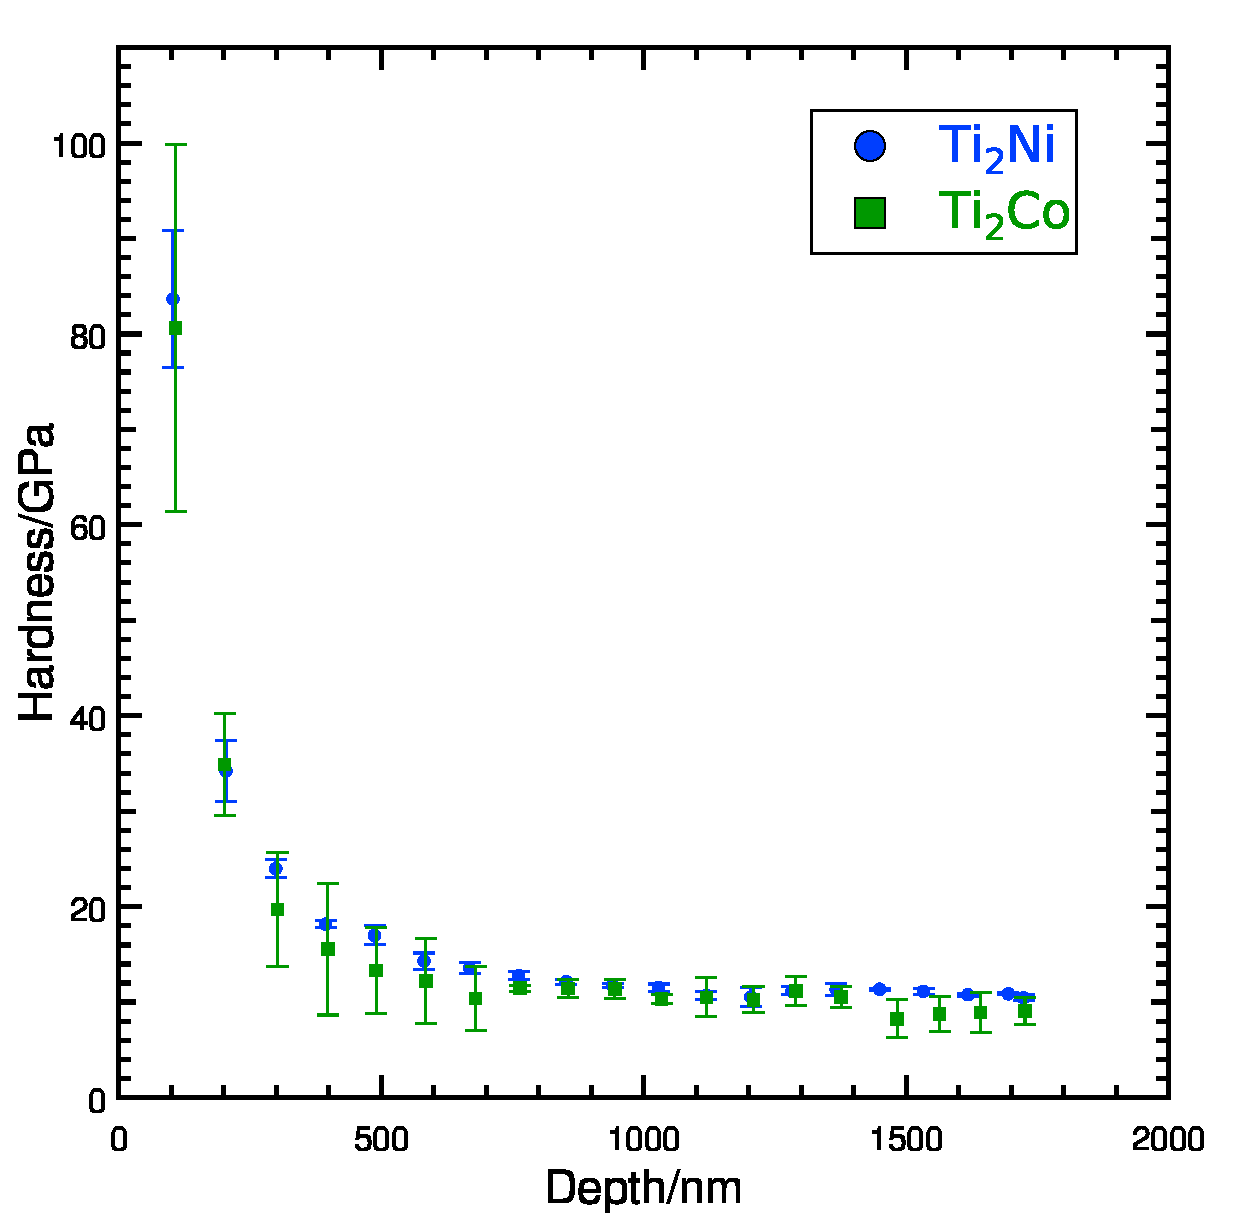
\includegraphics[width=0.7\textwidth]{Depth_vs_Hardness_Ti2Ni}
\caption[The size effect on indentation in \ce{Ti2Ni}]{The effect of indent depth (at maximum load) on the measured hardness for \ce{Ti2Ni} and \ce{Ti2Co} using a Berkovich indenter on a Micromaterials NanoTest rig. The hardness values are high at low depths as predicted by the size effect \cite{Cripps2011} and plateau at around \SI{800}{\nano\meter}.\label{fig:Depth_vs_hardness_Ti2Ni}}
\end{figure}














\FloatBarrier
\subsection{Slip system}
\FloatBarrier




A micropillar milled in \ce{Ti2Ni} was characterised with EBSD and compressed. The compressed pillar was imaged by SEM and shows slip traces on the surface. The micrographs are shown in \autoref{fig:micropillar}. The compression axis was found to be approximately parallel to the [1\,1\,6] direction. Slip traces developed on the surface of the micropillar as deformation occurred. There are two slip systems, of the expected type [1\,0\,\={1}](1\,1\,1), with the largest Schmid factor, the [1\,0\,1](\={1}\,1\,1) and the [0\,1\,1](1\,\={1}\,1), so the slip trace was examined to see if either of these slip systems match. This was done with the crystallographic visualisation package VESTA \cite{Momma2011,Momma2014} which can align unit cells to a known three dimensional orientation and show the orientation of lattice planes. The visualisations are also shown in \autoref{fig:micropillar} next to the corresponding view of the micropillar.

\begin{figure}[!h]
\centering
\begin{subfigure}{0.45\textwidth}
\centering
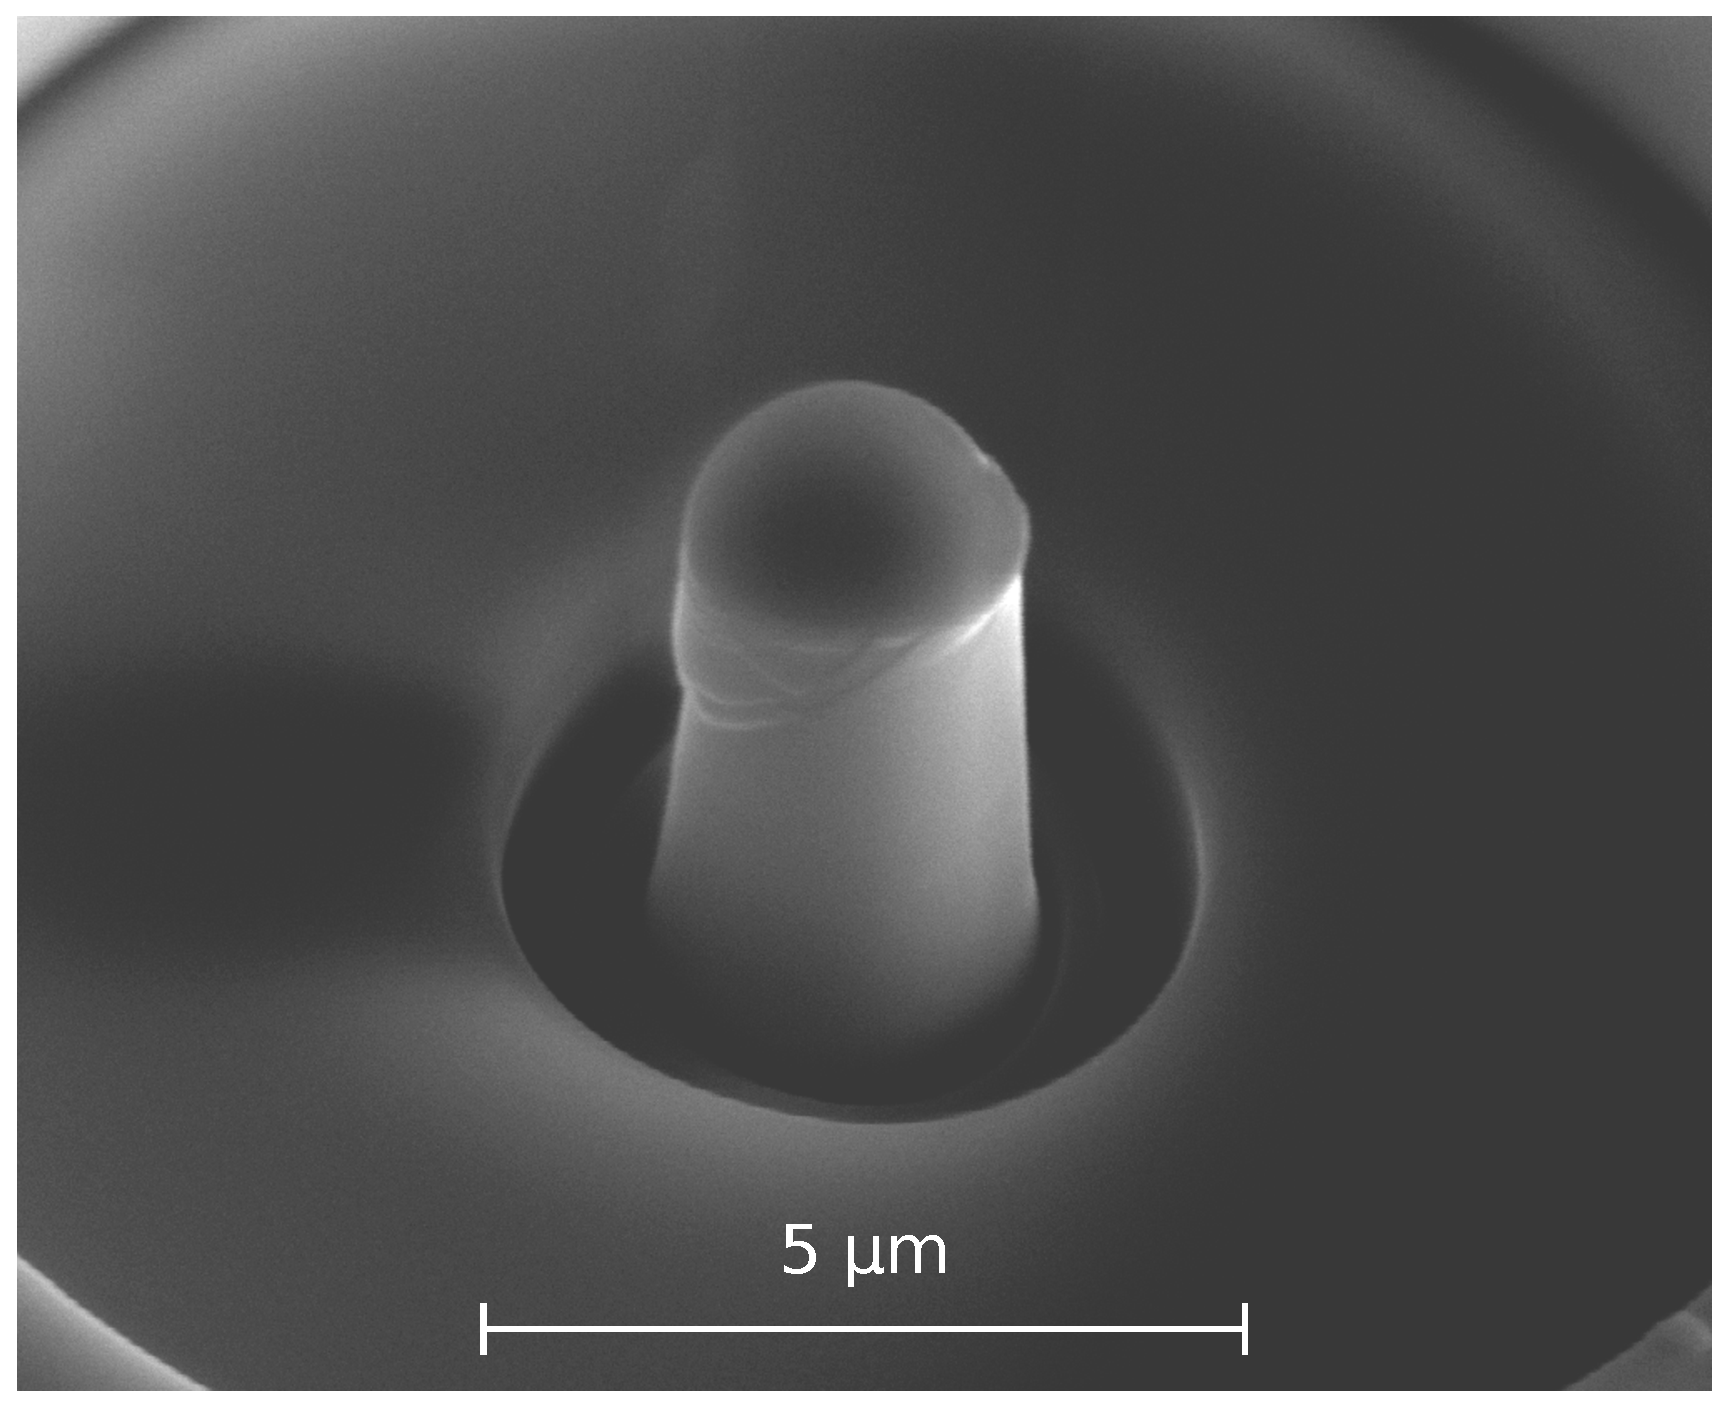
\includegraphics[width=0.8\textwidth]{pillar_3_v1}
\caption{First view of the compressed \ce{Ti2Ni} micropillar. The horizontal is approximately parallel to [0\,5\,\={1}]}
\end{subfigure}
~
\begin{subfigure}{0.45\textwidth}
\centering
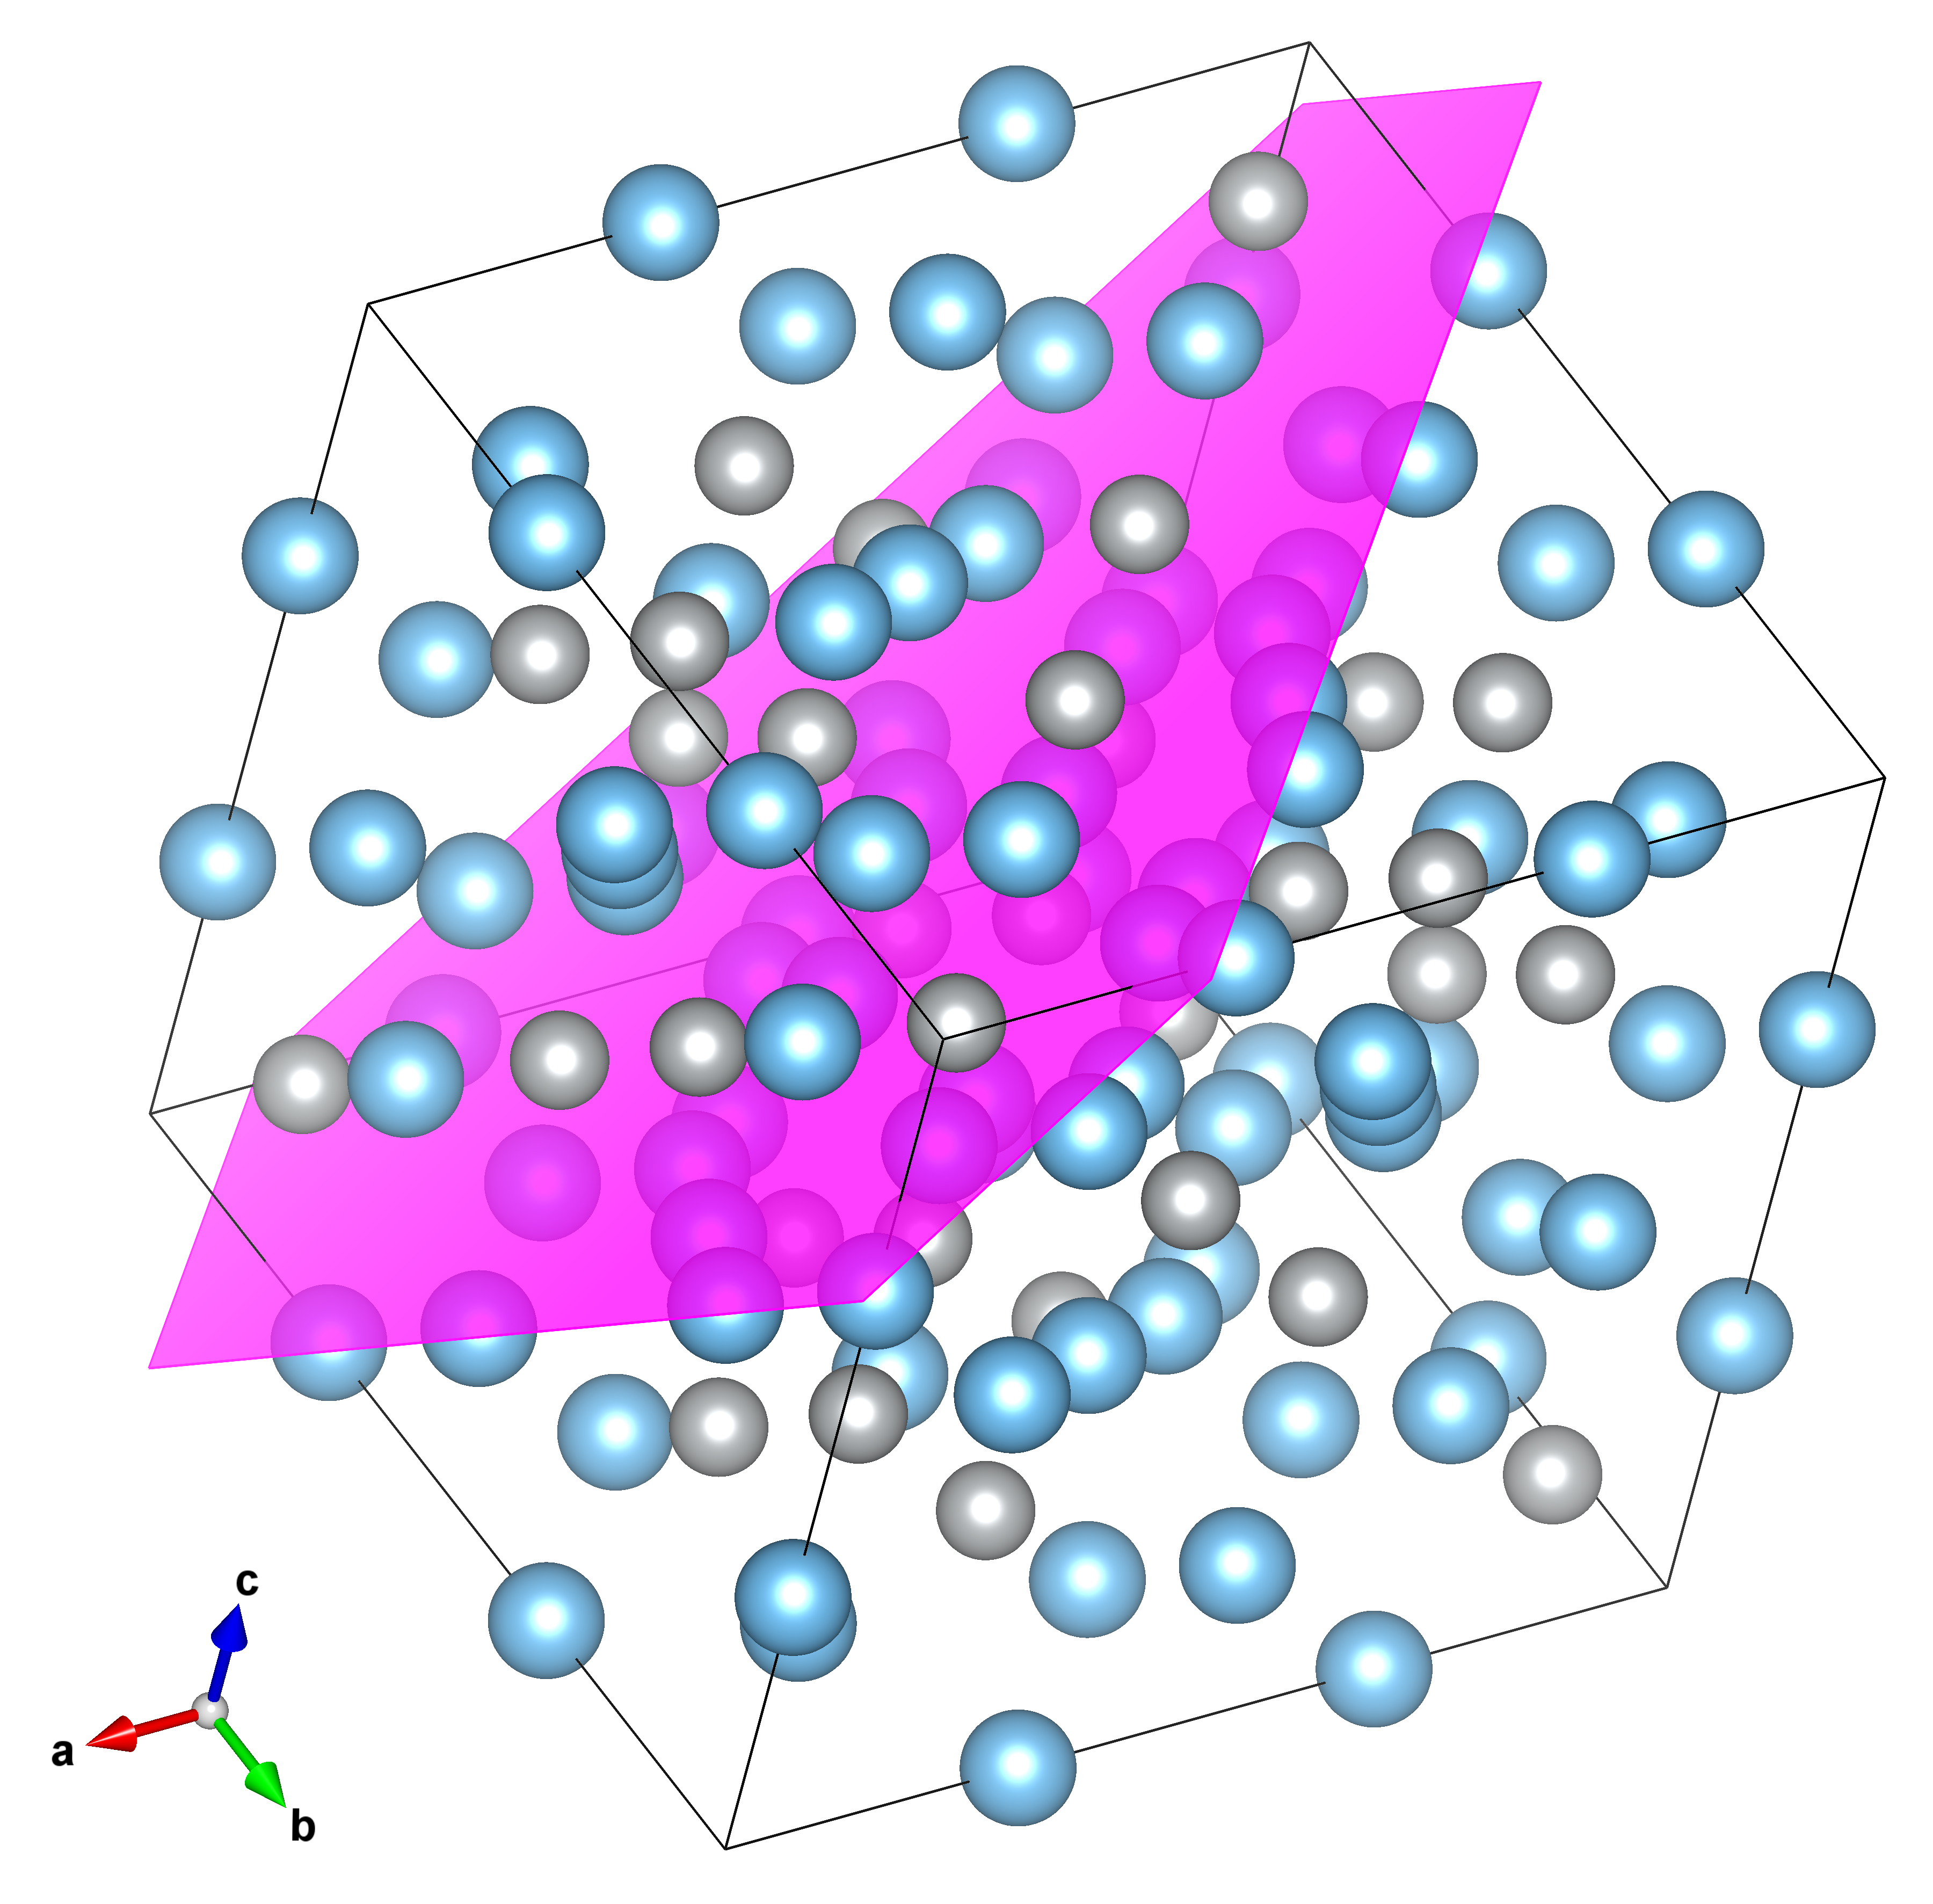
\includegraphics[width=0.66\textwidth]{Pillar_3_unit_cell_v1}
\caption{The unit cell aligned with the EBSD results for the first orientation showing the expected slip plane, (1\,\={1}\,1).}
\end{subfigure}
\par\bigskip
\begin{subfigure}{0.45\textwidth}
\centering
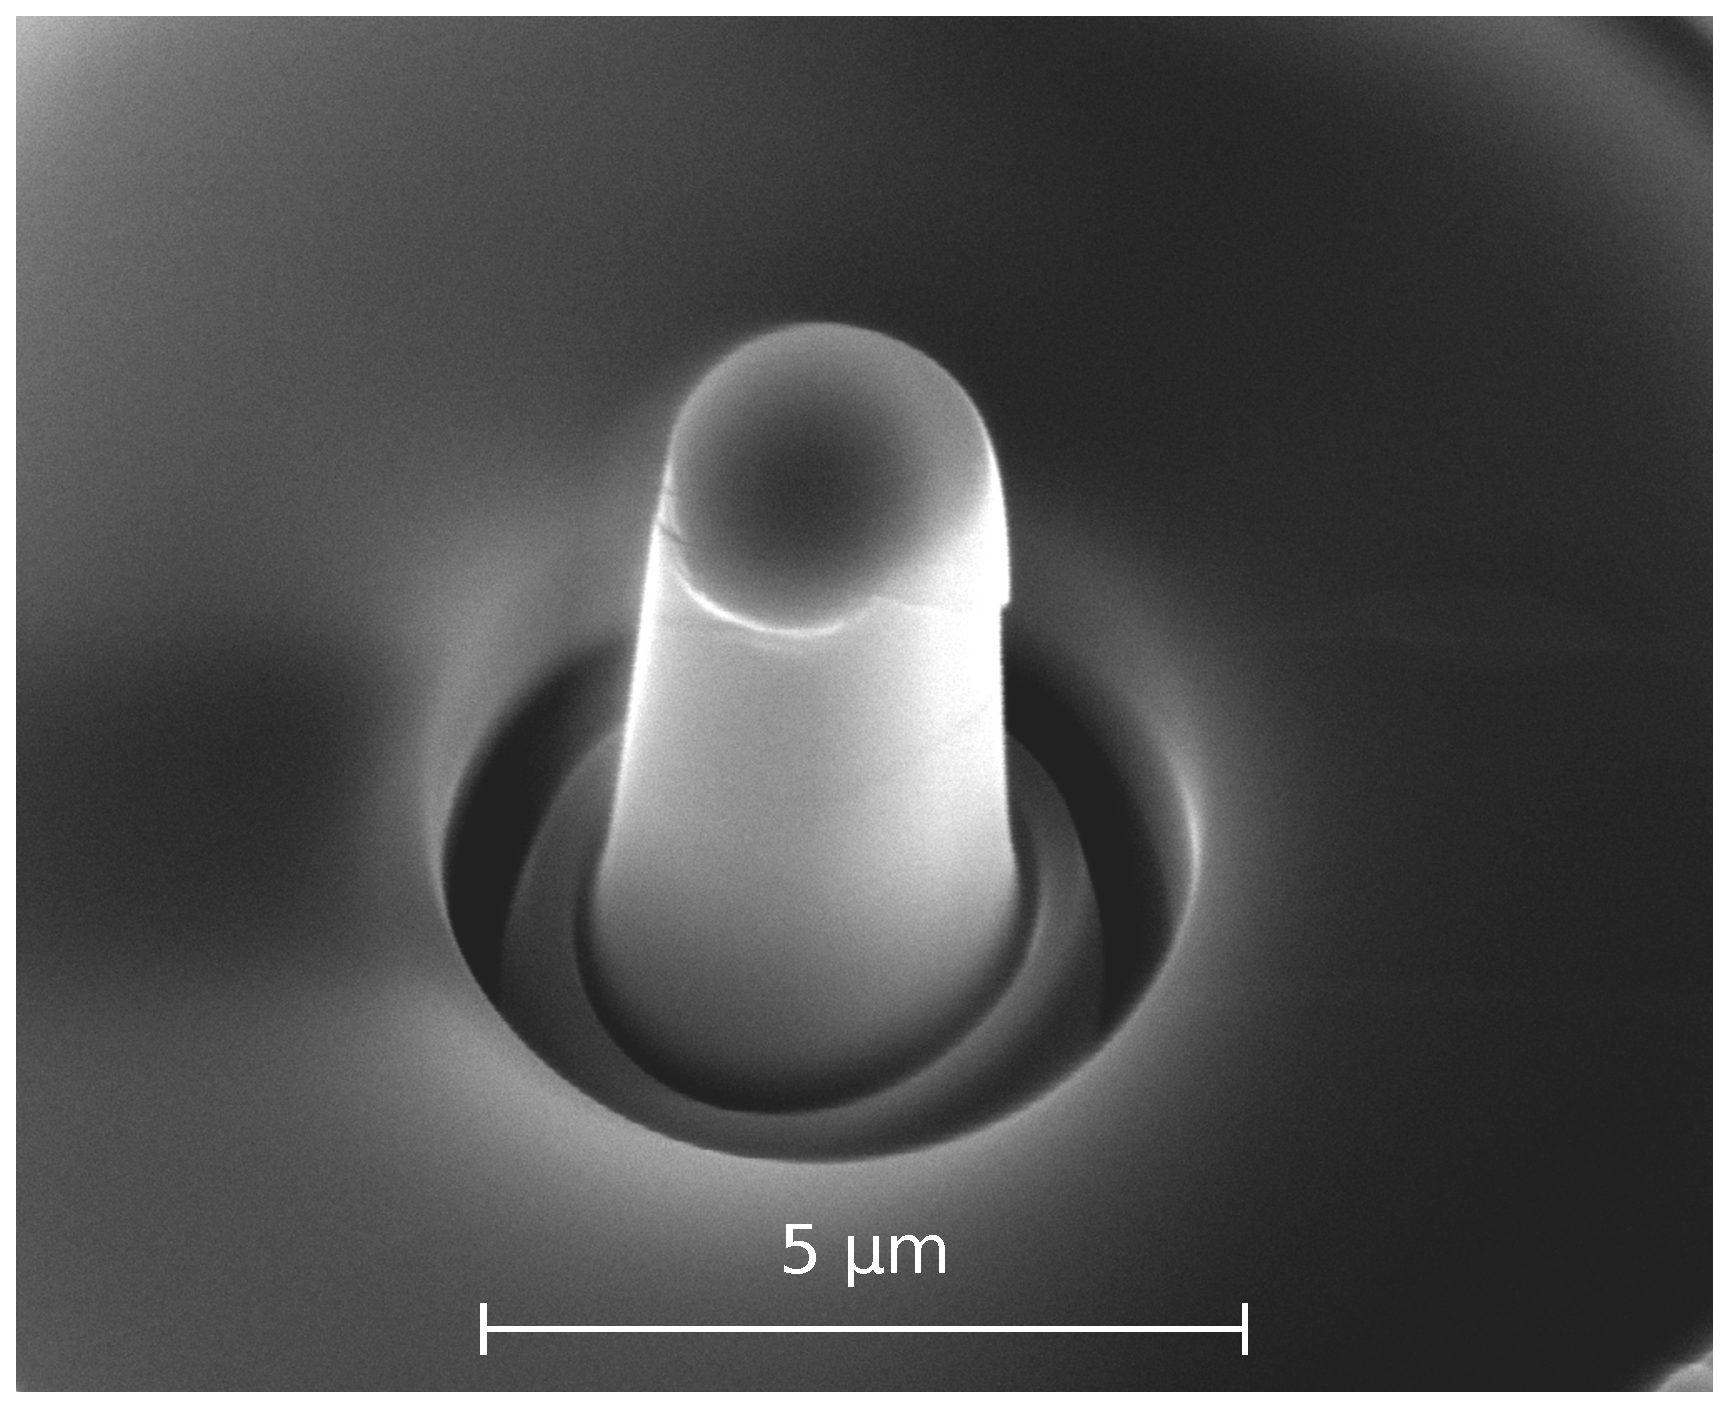
\includegraphics[width=0.8\textwidth]{pillar_3_v2}
\caption{Second view of the compressed \ce{Ti2Ni} micropillar. The horizontal is approximately parallel to [6\,0\,\={1}]}
\end{subfigure}
~
\begin{subfigure}{0.45\textwidth}
\centering
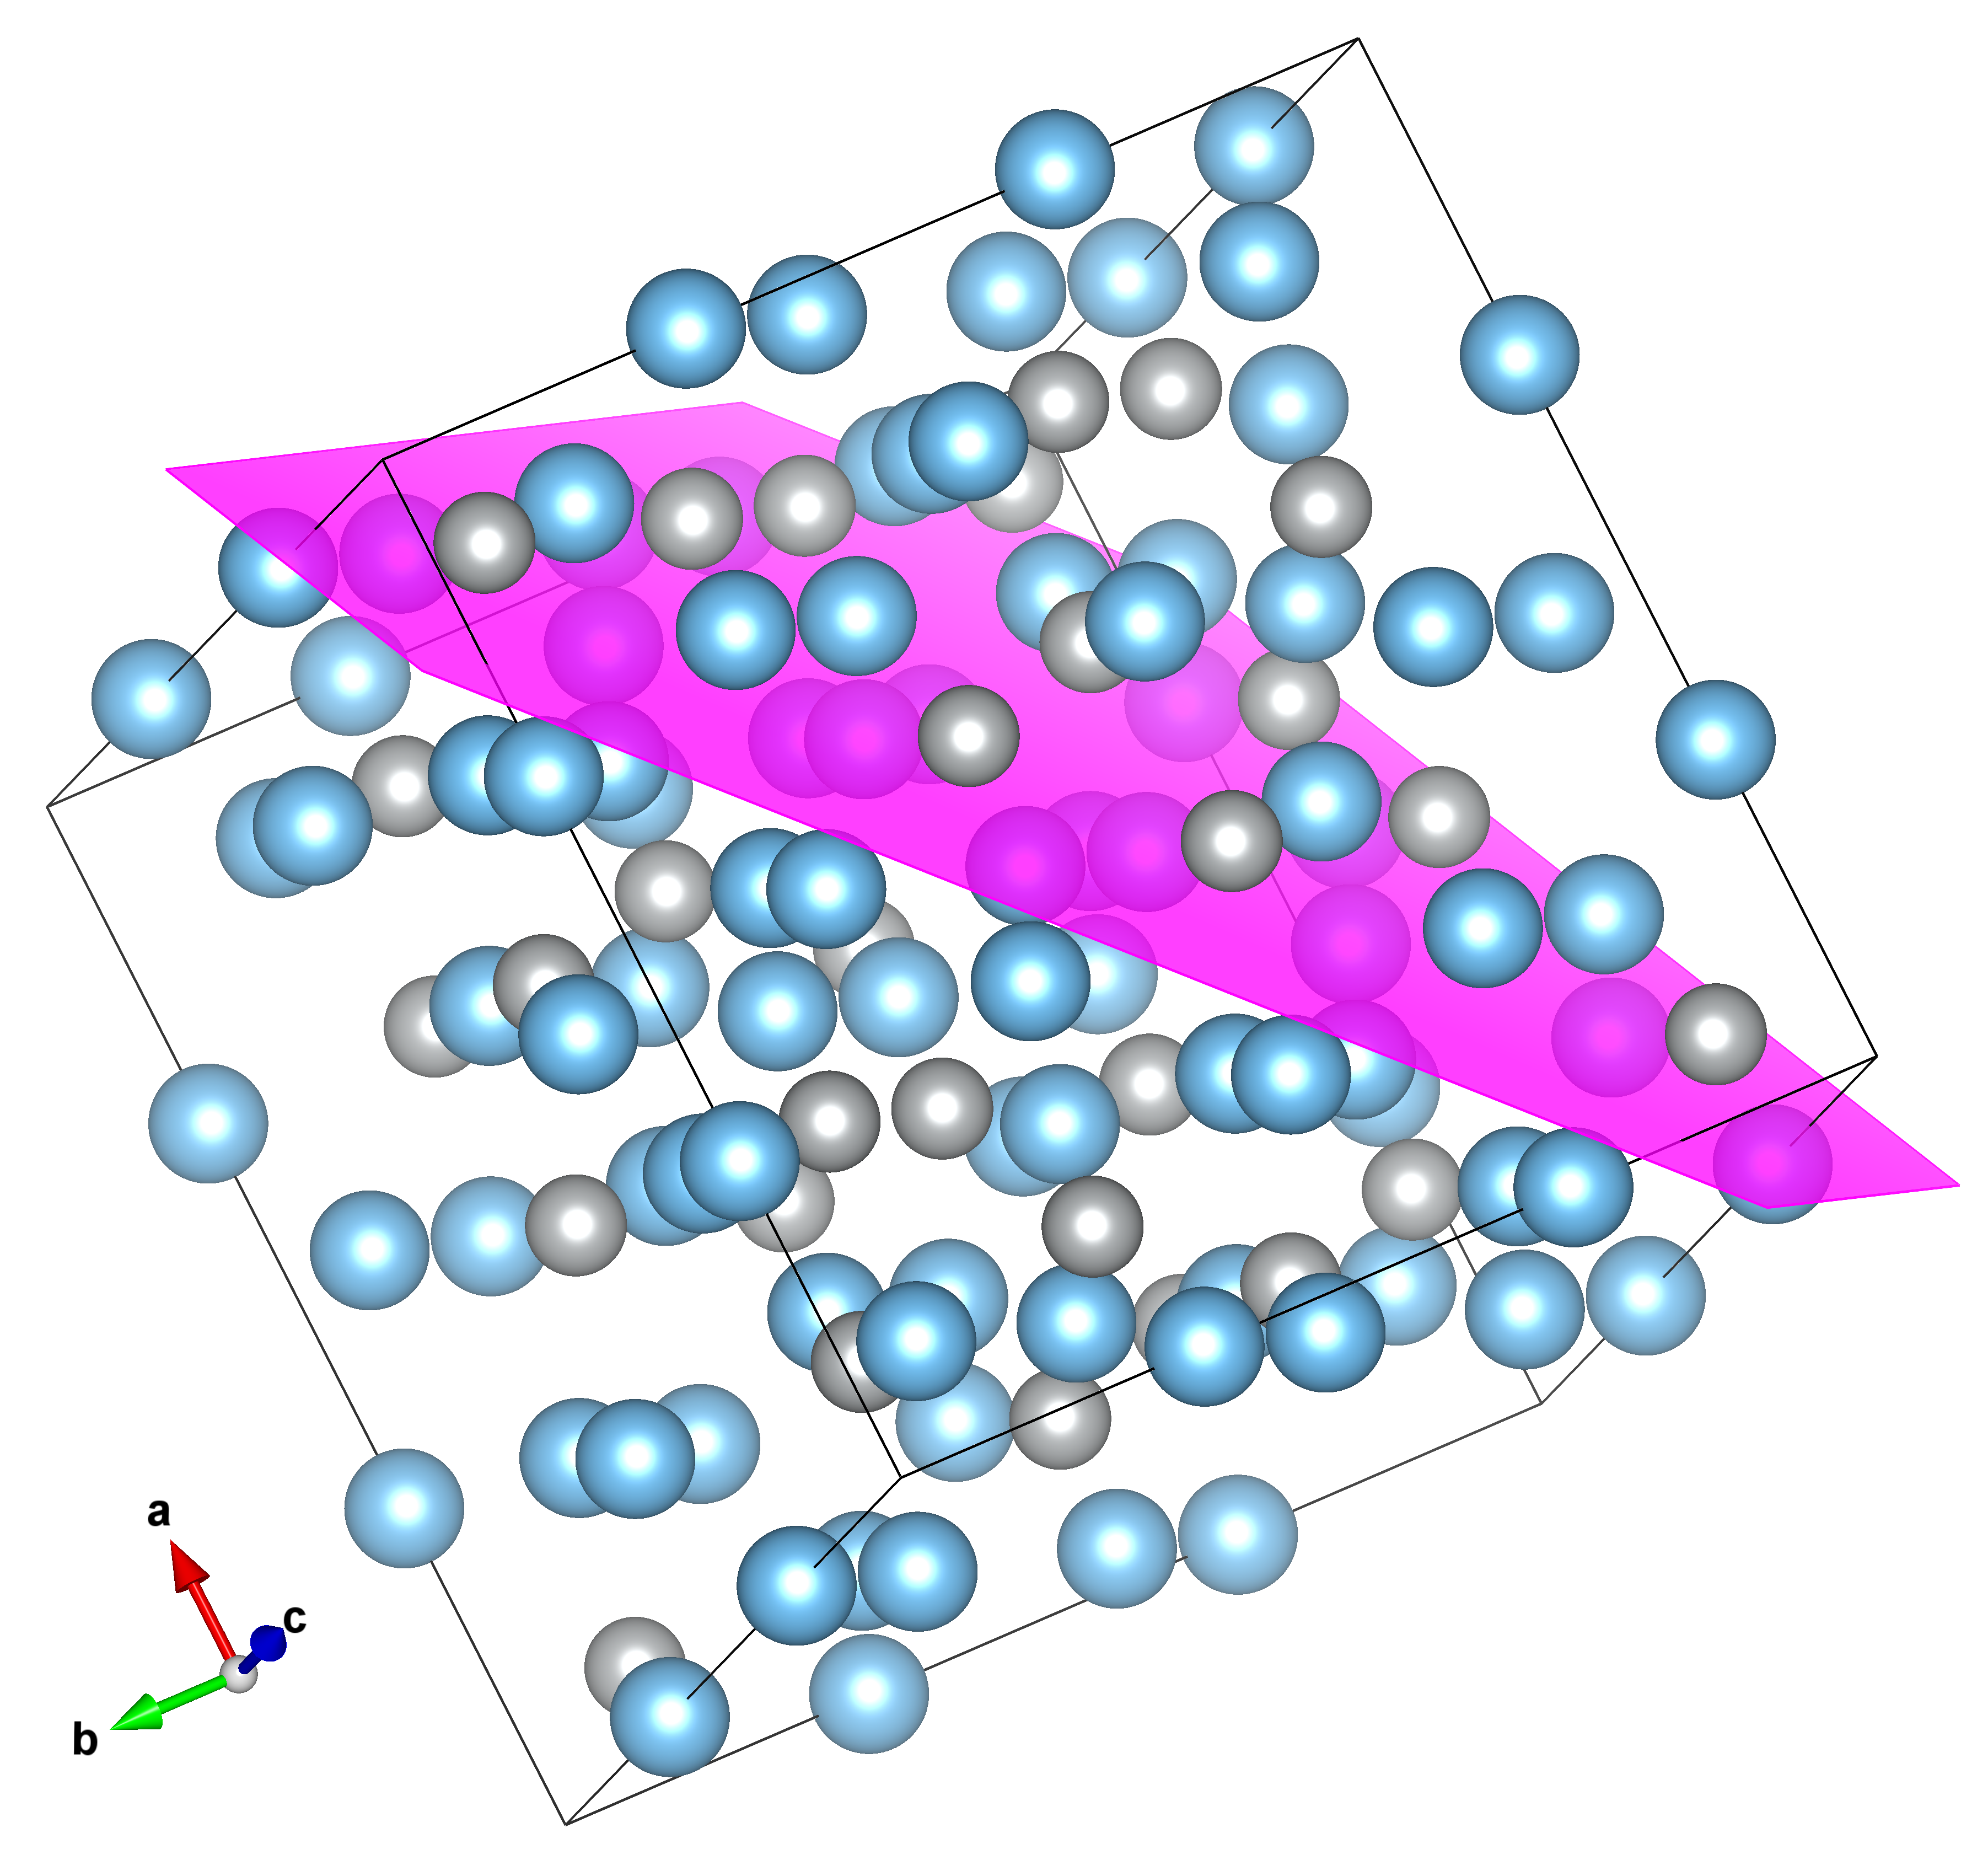
\includegraphics[width=0.66\textwidth]{Pillar_3_unit_cell_v2}
\caption{The unit cell aligned with the EBSD results for the second orientation showing the expected slip plane, (1\,\={1}\,1).}
\end{subfigure}
\caption[A compressed micropillar of \ce{Ti2Ni} showing the slip plane.]{A compressed micropillar in \ce{Ti2Ni} showing the expected slip plane, (1\,\={1}\,1), for the compression axis [1\,1\,6].\label{fig:micropillar}}
\end{figure}

The slip direction was difficult to identify from the pillar shown in \autoref{fig:micropillar} since relatively little displacement had occurred, to find the displacement a second micropillar was compressed to greater extent, shown in \autoref{fig:slip_direction}. This pillar has also slipped on a \{111\} plane. The observed slip direction is closer to the <2\,1\,1> than either of the <1\,1\,0> directions, so plastic flow is likely to be mediated by partial dislocations predominantly.

\begin{figure}
\centering
\begin{subfigure}{0.4\textwidth}
    \centering
    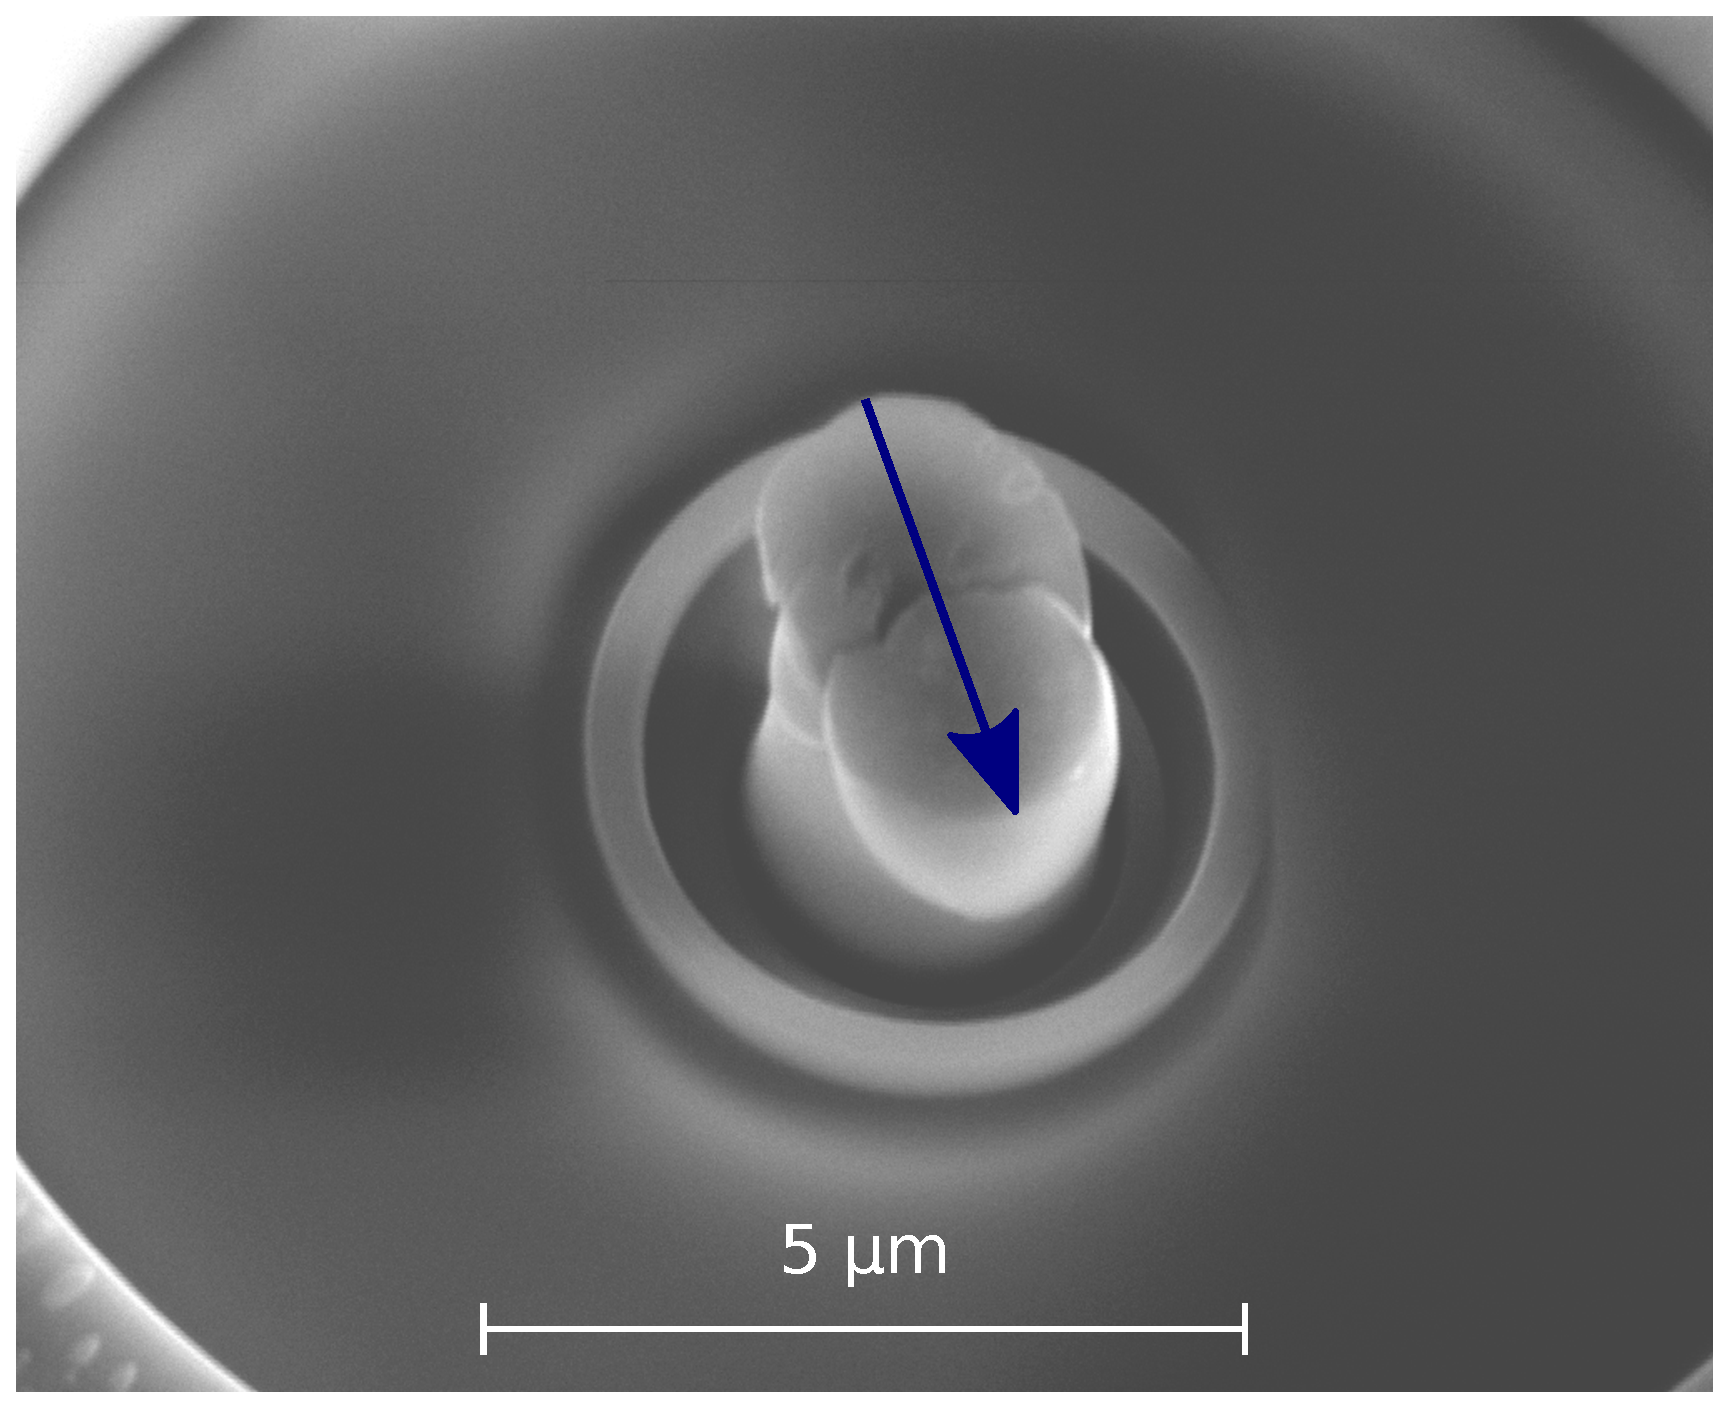
\includegraphics[width=\textwidth]{pillar_1_v1}
    \caption{A pillar with more deformation to show the slip direction more clearly.}
\end{subfigure}
~
\begin{subfigure}{0.4\textwidth}
    \centering
    \includegraphics[width=\textwidth]{pillar_1_v1_slip_directions}
    \caption{The expected slip plane  (1\,\={1}\,1) with three possible slip directions }
\end{subfigure}
\caption[A compressed micropillar of \ce{Ti2Ni} showing the slip direction.]{A micropillar compressed to a greater degree and the corresponding crystal lattice orientation obtained by EBSD. The compression axis was [3\,1\,6]. The slip plane matches the expected (1\,\={1}\,1) type and possible slip directions are shown in (b), the red arrows are <1\,1\,0> directions and the green arrow is the [2\,1\,1] direction.\label{fig:slip_direction}}
\end{figure}

This is an important result as it justifies the calculation for the electronegativity difference of the structure as the difference between the planes of atoms parallel to the \{1\,1\,1\}, as shown in \autoref{fig:slip_system_Ti2Ni}.






\FloatBarrier
\subsection{Hardness results}
\FloatBarrier


The hardness values for each phase are presented in \autoref{fig:hardness_vs_electronegativity} and summarised in \autoref{tab:hardness_ti2ni}. \autoref{fig:hardness_vs_electronegativity} shows that the increasing electronegativity difference has a substantial impact on the hardness of phases with the \ce{Ti2Ni} structure. As the electronegativity difference between the layers of the \ce{Ti2Ni} structure increases the measured hardness decreases, as expected by analogy with the MAX phases. 


\begin{figure}
\centering
\captionsetup{width=0.7\textwidth}
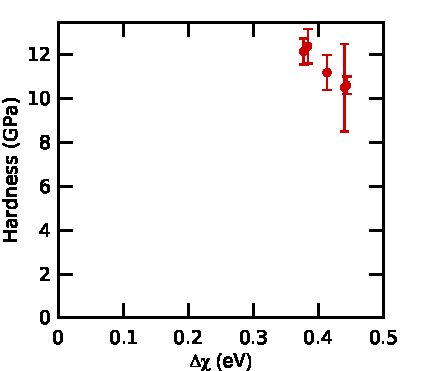
\includegraphics[width=0.7\textwidth]{dX_vs_hardness_Ti2Ni}
\caption[The variation of hardness with electronegativity difference in the \ce{Ti2Ni} structure.]{The variation of hardness, as measured with a Berkovich indenter, with electronegativity (Mulliken scale \cite{Mulliken1934}), a reduction in hardness of almost \SI{2}{\giga\pascal} or \SI{16}{\percent} is seen for a modest variation in electronegativity.\label{fig:hardness_vs_electronegativity}}
\end{figure}

\begin{table}
\centering
\begin{tabular}{| l | c | c | c | c |}
\hline
Stoichiometry & Hardness (\si{\giga\pascal}) & Std. Dev. (\si{\giga\pascal}) & n & $\Delta \chi$ (\si{\electronvolt}) \\
\hline
\ce{Ti2Ni} \rule{0pt}{3ex}               & 10.61 & 0.38 & 30 & 0.444 \\ % the strut adds a little space at the top of the table
\ce{(Hf,Ti)_{2}Ni}                       & 10.61 & 0.55 & 10 & 0.440 \\
\ce{Ti2(Co,Ni)}                          & 11.28 & 0.68 & 17 & 0.414 \\
\ce{Ti2Co}                               & 12.42 & 0.75 & 9  & 0.383 \\
\ce{Hf2Co} \rule[-1ex]{0pt}{0pt}         & 12.54 & 0.36 & 12 & 0.378 \\ % strut adds a little space after the line
\hline
\end{tabular}
\caption{\rule{0pt}{3ex}The hardness results for the different stoichiometries with the \ce{Ti2Ni} structure.\label{tab:hardness_ti2ni}}
\end{table}


All the stoichiometries tested are hard, but a substantial variation was observed, the hardness was between \num{10.6} and \SI{12.6}{\giga\pascal}. The substitution of nickel with cobalt produced the biggest change in hardness, for example between \ce{Ti2Ni} and \ce{Ti2Co} the hardness drops \SI{1.81}{\giga\pascal}, or \SI{14.6}{\percent}, from \SI{12.42}{\giga\pascal} to \SI{10.61}{\giga\pascal}, as might be expected given the change in electronegativity difference this substitution gives rise to. The substitution of hafnium for titanium has a smaller effect on the electronegativity difference between the layers and a correspondingly smaller effect on the hardness, \ce{Ti2Co} and \ce{Hf2Co} differ by \SI{0.12}{\giga\pascal}, which is of the order of the error in the hardness measurement. In the case of \ce{Ti2Ni} and \ce{(Hf,Ti)_{2}Ni} there is no measured change in the hardness in either direction, which might be expected for the small change in the electronegativity difference, less than \SI{0.01}{\electronvolt}. The mixed stoichiometries, \ce{Ti2(Co,Ni)} and \ce{(Hf,Ti)_{2}Ni} fit the trend well and do not exhibit any solution hardening as might be expected. Particularly noteworthy is that \ce{Ti2(Co,Ni)} has an intermediate value of electronegativity difference and falls exactly on the trend between the the extreme cases.





\section{Conclusions}


The heterogeneity at the unit cell level has been explored in phases with the face-centred cubic \ce{Ti2Ni} structure. The crystallography of the structure was examined and the likely heterogeneous regions identified as the planes parallel to the \{1\,1\,1\}. These planes are made up of strongly bound clusters at the 16(c) position, which form a Kagom\'{e} network. The electronegativity difference between the regions of the unit cell was found to be likely to strengthen the bonding of this network, containing atoms like nickel and cobalt on the 16(c) site. Stoichiometries were identified to explore a range electronegativity differences using the elements Hf, Ti, Ni and Co, varying $\Delta \chi$ over the range \SIrange{0.378}{0.444}{eV}.

The slip system in the \ce{Ti2Ni} was characterised by the compression of micropillars with a known crystallographic orientation as determined by EBSD. The slip plane was found to be the \{1\,1\,1\} and the slip direction was found to be closest to <2\,1\,1>, implying that slip is predominantly mediate by partial dislocations, which is to be expected in a material for which the Burgers vector is so large.

Hardness measurements by instrumented nanoindentation was undertaken to characterise the size effect, which was shown to be limited to indents with a depth less than approximately \SI{800}{\nano\meter}. Further indents were made on known crystallographic faces of the crystal to determine a proxy metric for the flow stress. The orientation was fixed to ensure that the effects of changing Schmid factors were minimised. The hardness was shown to vary significantly with changing electronegativity, a modest change in $\Delta \chi$ of \SI{0.066}{\electronvolt} produced a softening of \SI{1.93}{\giga\pascal}, or \SI{15.4}{\percent} 

Though more modest in scale than the effects seen in the MAX phases, where the range of $\Delta \chi$ is \SIrange{0.02}{1.59}{\electronvolt}, the \ce{Ti2Ni} structure has demonstrated the same heterogeneity softening; hardness decreases as the composition is varied to increase the heterogeneity within the unit cell. This demonstrates the effect in a cubic structure, which is not limited to a small number of slip systems like the hexagonal MAX phases, suggesting that elastic heterogeneity offers a route to tailoring the ductility and thereby the toughness of non-metallic materials.
















































